\documentclass{jarticle}

\usepackage{tam}
\usepackage{fleqn}
\usepackage{url}
\usepackage{bm}
\usepackage[dvipdfmx]{graphicx}
\usepackage[dvipdfmx]{color}
%\usepackage{color}
\usepackage{colordef}
\usepackage{amssymb}
\usepackage{pdfpages}
\usepackage{amsmath}

%%%%%%%%%% Command alias %%%%%%%%%%
\newcommand{\IB}{$\bullet$}
\newcommand{\IC}{$\circ$}
\newcommand{\IS}{$*$}
%%%%%%%%%%%%%%%%%%%%%%%%%%%%%%%%%%%

\title{デマンド電力を考慮した電力運用最適化問題を動的計画法で}
\author{神戸大学大学院 奥村侑真}
\date{}

\def\baselinestretch{1.02}
\renewcommand{\thefootnote}{\roman{footnote}}

\begin{document}
\maketitle


\section{託送を動的計画法で反映させるには}
\subsection{定式化}
前述の問題にフードテクノ様からの要求である「デマンド電力をなるべく小さくする」という要素を加えることを考える．このとき問題は以下のような形になる．なお$p^{\rm B}$は
基本料金単価(単位は円/kW)を表す．
\begin{equation}
    \text{Minimize} \quad \{ p^{\rm B}\max_{k} s_k^{\rm BY}(s_{i},s_{j}) \} +  \sum_{k=0}^{K-1} w_k(s_i,s_j) \quad s_i \in S_k, s_j \in S_{k+1}, -a^{\rm SL}  \leq s_k^{\rm {BY}}(s_i,s_j)  \leq a^{\rm BY} 
 \label{eq:minimize}
\end{equation}


\subsection{最適性の原理に関する議論}
本問題を，残りの条件式や変数の定義の仕方，状態，状態遷移の候補の決め方などを上記と同様にした場合，”最適経路の部分経路もまた最適でなければならない”という最適性の原理を満たしていないため，動的計画法で解くことができない．
以下，最適性の原理を満たさないケースの例として\\
$K = 4，\\
\overline{b} = 2,B = 3，i_{0} = 0，\\p_{1}^{\rm BY} = 5,p_{2}^{\rm BY} = 1，p_{3}^{\rm BY} = 1，p_{k}^{\rm SL} = 0，p^{\rm B} = 100，\\ 
\alpha^{\rm P} = \alpha^{\rm DA}=\alpha^{\rm DB}=\alpha^{\rm DC}=\alpha^{\rm FC} = \alpha^{\rm FD} = 1，\\
g_{1}^{\rm P1} - d_{1}^{\rm A2} - d_{1}^{\rm B2} - d_{1}^{\rm C2} = 0,g_{2}^{\rm P1} - d_{2}^{\rm A2} - d_{2}^{\rm B2} - d_{2}^{\rm C2} = 0,g_{3}^{\rm P1} - d_{3}^{\rm A2} - d_{3}^{\rm B2} - d_{3}^{\rm C2} = -5，\\
a^{\rm BY} = a^{\rm SL} = 100$\\
を満たす場合について考える．このとき，目的関数は次のように表される．
\begin{equation}
    \text{Minimize} \quad \{ 100\max_{k} s_k^{\rm BY}(s_{i},s_{j}) \} +  \sum_{k=0}^{3} w_k(s_i,s_j) \quad s_i \in S_k, s_j \in S_{k+1}
 \label{eq:minimize}
\end{equation}

この場合について，とりうる状態と状態遷移を図にしたものを図\ref{fig:network_hanrei}に示す．なお，赤の数字はその状態遷移での買電量，すなわち,$s_{k}^{\rm BY}(s_i,s_j)$を表し，青の数字はその状態遷移での買電価格，すなわち，$w_k(s_i,s_j)$を表す．
このとき，$s_0(\in S_0)$から$s_2(\in S_3)$へ向かうための最適経路を考えると，黒色の太線になる(この経路の評価値は$\max_{k} s_k^{\rm BY}(s_{i},s_{j}) = 5, \sum_{k=0}^{3} w_k(s_i,s_j) = 7$より507となる)．この最適経路の部分経路である，$s_0(\in S_0) ，s_0(\in S_1)，s_2(\in S_2)$の状態遷移を結ぶ経路に注目すると，この経路は$s_0(\in S_0)$から$s_2(\in S_2)$へ向かうための最適経路最適経路にならなくてはならない(この部分経路の評価値は202)．ところが，この経路よりも良い経路である，$s_0(\in S_0) ，s_1(\in S_1)，s_2(\in S_2)$の状態遷移を結ぶ経路が存在する(この部分経路の評価値は106)．よって，最適性の原理を満たさず，このままだと動的計画法による求解はできない．この問題を動的計画法で解くためには，状態の決め方を変え，最適性の原理を満たすようにしなければならない．例えば，「状態$s_i (\in S_k)$を期$k$の末尾におけるバッテリーのSOCが$i$段階である状態」と定義するのではなく，「状態$s_{i,j}(\in S_k)$を期$k$の末尾におけるバッテリーのSOCが$i$段階かつ期0から期$k$までの各期の中で最大の買電電力量が$j$である状態」と定義するなどすれば最適性の原理を満たすようになる．ところがこの場合，状態遷移の数が($j$を離散的に刻んだ数)倍だけ増加するため，求解にかなりの時間がかかってしまうことが想定される．逆に動的計画法ではなく，線形計画法でデマンド電力を考慮する場合については，後述する手法により目的関数を線形化することができるため，線形計画法の方が実装が容易であると考えられる．

\subsection{デマンド電力を線形計画法で扱うには}
目的関数が\\
Minimize
\begin{equation}
    \max (x_1,x_2,\dots , x_n) + 2y
\end{equation}
のような項が存在する場合，その項は非線形であり求解が困難となる．そのため，この項を線形化することを考える．具体的には新たな変数をひとつ導入し，\\
Minimize
\begin{equation}
    z + 2y
\end{equation}
Sub.to
\begin{equation}
    x_1 \leq z
\end{equation}
\begin{equation}
    x_2 \leq z
\end{equation}
    \dots \\
\begin{equation}
    x_n \leq z
\end{equation}

とすることにより線形化することができ，求解が容易に可能となる．

\begin{figure}[h]
 \centering
 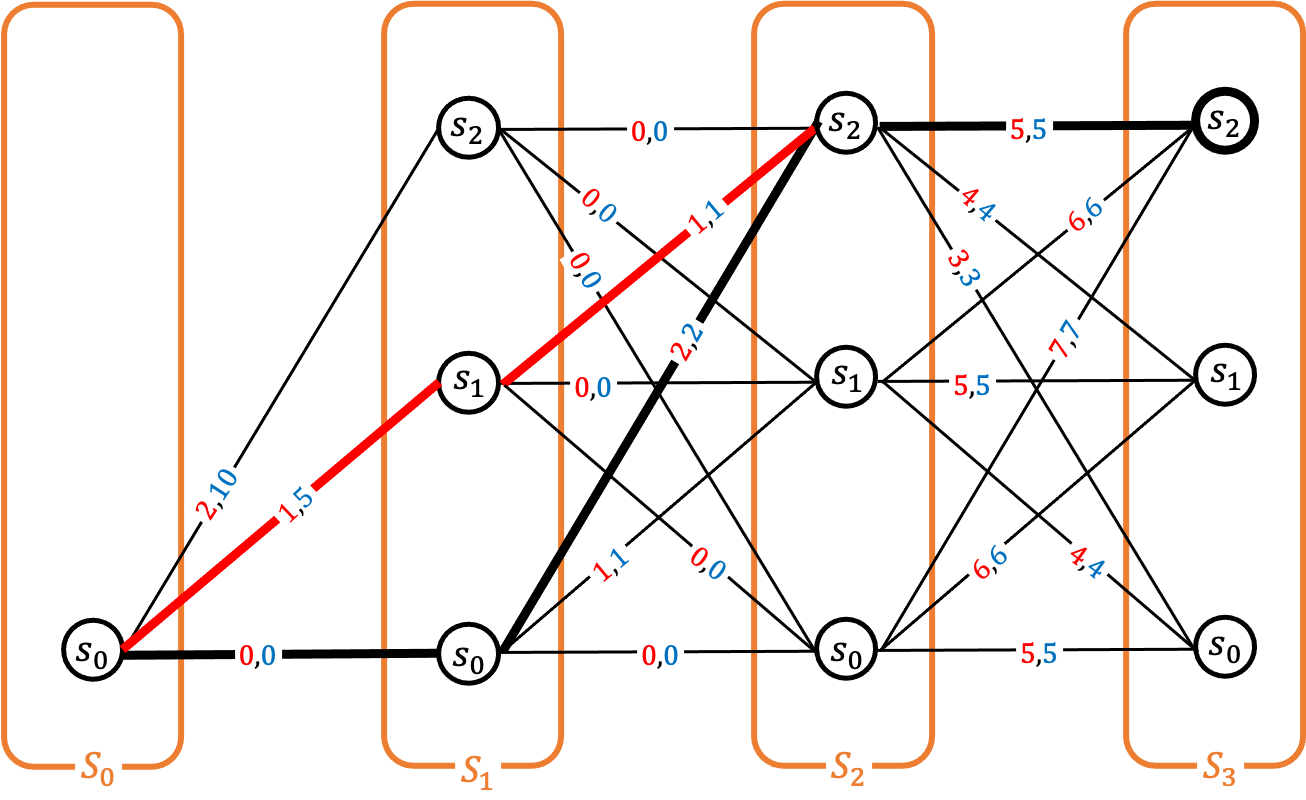
\includegraphics[width=145mm]{../figure/network_hanrei.png}
 \caption{最適性の原理を満たさない例}
 \label{fig:network_hanrei}
\end{figure}






\end{document}
